% =============================================================================
% Kapitel 4: Failure Cases
% =============================================================================

\section{Failure Cases}
\label{sec:cases}

Dieses Kapitel stellt die fünf untersuchten Failure Cases dar. Jeder Case erläutert den
relevanten Systemkontext und die zugrunde liegende Schwachstelle, beschreibt das gemessene
Verhalten und leitet daraus Interpretation und Handlungsempfehlung ab.

% Hinweis: Pflicht "mind. eine Grafik" ist durch die zwei Mess-Plots (Abb. \ref{fig:case2},
% \ref{fig:case3}) bereits erfüllt. Optional kann zusätzlich ein Architekturdiagramm der
% Prozess-Topologie in Kap. \ref{sec:einleitung} oder \ref{sec:methodik} ergänzt werden
% (Quelle: sammelsorium/misc/Process-Diagram.png bzw. eigene Darstellung aus Pipeline.md).

\subsection{Case 1 -- Lücken in der Laufzeit-Prozesssupervision}
\label{sec:case1}

Im stationären Betrieb überwacht das System ausschließlich den \texttt{PipelineManager}
über einen Poll im Sekundentakt. Die drei weiteren Service-Prozesse für Frame-Grabbing,
Datenbereitstellung und Logging laufen nach erfolgreichem Start ohne jede
Laufzeitüberwachung; eine Supervisor-Logik im Sinne von
Abschnitt~\ref{sec:grundlagen-supervision} existiert nicht. Um die Auswirkung dieser
Lücke zu quantifizieren, wurde jeder Service-Prozess einzeln per \texttt{SIGKILL} zum
Absturz gebracht. Tabelle~\ref{tab:case1} zeigt, ob der Hauptprozess den Ausfall erkennt
und welche Systemreaktion daraus folgt.

\begin{table}[htbp]
    \centering
    \caption{Erkennung von Service-Prozess-Ausfällen}
    \label{tab:case1}
    \begin{tabularx}{\textwidth}{lllX}
        \hline
        \textbf{Zielprozess} & \textbf{Erkannt} & \textbf{TTD} & \textbf{Systemreaktion} \\
        \hline
        PipelineManager  & ja   & 0,992\,s & geordneter Shutdown aller Subsysteme \\
        FrameGrabber     & nein & --       & Deadlock in Pipeline-Schritt 1 \\
        InspDataHandler  & nein & --       & stiller Ausfall, laufende Inspektionen enden \\
        Logger           & nein & --       & stiller Ausfall, kein Log-Output mehr \\
        \hline
    \end{tabularx}
\end{table}

Die Tabelle macht die zentrale Schwachstelle sichtbar: Nur der Prozess, der in der
Hauptschleife abgefragt wird, löst eine Reaktion aus. Alle anderen Ausfälle bleiben im
Beobachtungsfenster ohne technische Meldung. Beim FrameGrabber ist die Folge ein
Pipeline-Stillstand in Schritt~1, weil keine neuen Bilddaten eintreffen. Beim
InspectionDataHandler und beim Logger läuft das System zunächst weiter, verliert aber
Datenbereitstellung beziehungsweise Protokollierung. Die Ausfälle entsprechen damit dem
Fail-Silent-Verhalten \cite{cristian1991}. Abhilfe schafft eine Überwachung aller
Service-Prozesse oder eine externe Supervision, etwa über eine \texttt{systemd}-Unit mit
\texttt{Restart=on-failure}.

\subsection{Case 2 -- Flüchtiger Bildspeicher als Single Point of Failure}
\label{sec:case2}

Verarbeitete Bilder werden auf einer als tmpfs-RAM-Disk gemounteten Partition abgelegt.
Die zuständige Funktion \texttt{store\_images\_to\_disk} enthält keine Fehlerbehandlung für
\texttt{OSError}, und der Füllstand wird nicht überwacht. Da eine RAM-Disk auf eine feste
Größe begrenzt ist (Abschnitt~\ref{sec:grundlagen-ressourcen}), schlagen
Schreiboperationen bei Erschöpfung fehl. Im Normalbetrieb wächst das Bildverzeichnis um
rund 21,8~MB pro Inspektion, was bei Produktionsdurchsatz einer Schreibrate von etwa
38~MB/s entspricht. Bei 12~GB freiem Speicher wäre die RAM-Disk damit nach ungefähr fünf
Minuten erschöpft, sofern keine Rotation oder Auslagerung greift. Abbildung~\ref{fig:case2}
ordnet die Messung ein: Schon der kurze Referenzlauf zeigt lineares Wachstum des
Bildverzeichnisses; ohne Begrenzung wird daraus im Dauerbetrieb ein Ausfallpunkt. Zur
Analyse des Fehlerfalls wurde eine volle Disk durch das gezielte Auslösen eines
\texttt{OSError(28)} nachgebildet (Tabelle~\ref{tab:case2}).

\begin{table}[htbp]
    \centering
    \caption{Verhalten bei erschöpftem Bildspeicher}
    \label{tab:case2}
    \begin{tabularx}{\textwidth}{lX}
        \hline
        \textbf{Messgröße} & \textbf{Wert} \\
        \hline
        Schreibrate (Hochrechnung Produktionslast) & $\approx$ 38 MB/s \\
        Zeit von \texttt{OSError} bis PM-Absturz   & 35,2 s \\
        PM-Absturz bis Shutdown                    & 2,1 s \\
        Graceful Degradation                       & nein \\
        \hline
    \end{tabularx}
\end{table}

\begin{figure}[htbp]
    \centering
    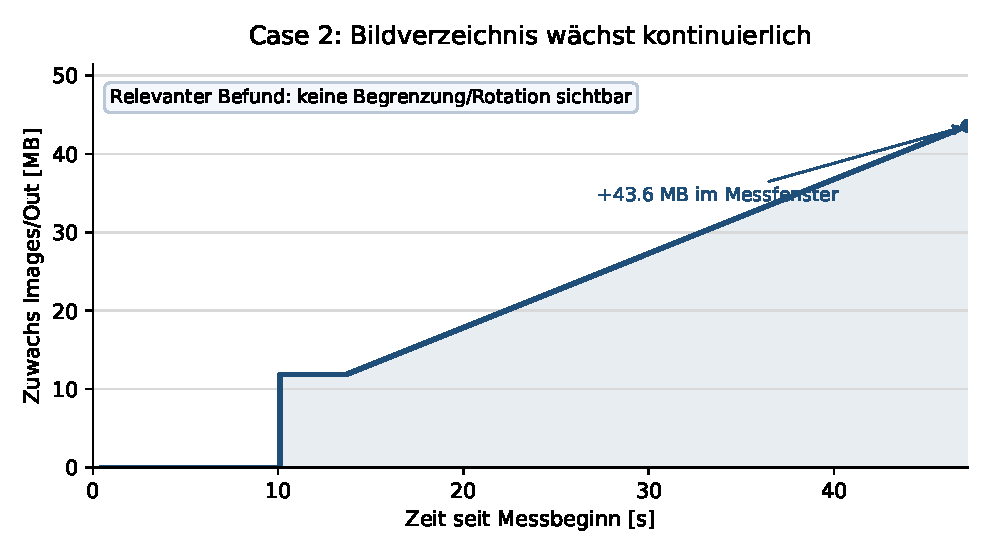
\includegraphics[width=0.85\textwidth]{assets/img/case2_image_out_usage.pdf}
    \caption[Wachstum des Bildverzeichnisses]{Wachstum des Bildverzeichnisses
        \texttt{Images/Out} im Referenzlauf. Der lineare Anstieg ist der relevante
        Befund; in Produktion liegt dieser Pfad auf einer begrenzten RAM-Disk.}
    \source{Eigene Darstellung auf Basis eigener Messdaten}
    \label{fig:case2}
\end{figure}

Ein einzelner fehlgeschlagener Schreibvorgang beendet den produktiven Ablauf. Zwischen
dem Fehler und dem erkannten Absturz liegt eine Stillstandsphase von gut 35~Sekunden, in
der der PipelineManager auf das Ergebnis des abgestürzten Workers wartet. Die RAM-Disk ist
damit ein einzelner Ausfallpunkt ohne Rückfallebene. Shared-Memory-Blöcke und Bildarchiv
liegen zwar auf unterschiedlichen Pfaden, nutzen aber denselben physischen Arbeitsspeicher.
Eine Fehlerbehandlung in \texttt{store\_images\_to\_disk}, die bei vollem Bildspeicher nur
die Archivierung überspringt, sowie ein Füllstands-Monitoring mit Alarm unterhalb von
20\,\% freiem Speicher würden diesen Ausfall verhindern.

\subsection{Case 3 -- Log-Queue-Stau als Pipeline-Blocker}
\label{sec:case3}

Alle Worker und der PipelineManager schreiben Log-Einträge synchron über
\texttt{log\_\allowbreak{}queue.\allowbreak{}put()} in eine zentrale, auf 1000 Einträge
begrenzte Queue. Der Aufruf
erfolgt blockierend ohne Timeout, und der Zustand \texttt{queue.Full} wird nicht abgefangen
-- eine Konstruktion, die Backpressure im Sinne von Abschnitt~\ref{sec:grundlagen-ressourcen}
erzeugt. Um eine hängende Datenbankschicht nachzubilden, wurde der Logger per
\texttt{SIGSTOP} eingefroren (Tabelle~\ref{tab:case3}).

\begin{table}[htbp]
    \centering
    \caption{Verhalten bei eingefrorenem Logger-Prozess}
    \label{tab:case3}
    \begin{tabularx}{\textwidth}{lX}
        \hline
        \textbf{Messgröße} & \textbf{Wert} \\
        \hline
        Durchsatz vor Eingriff             & 17 Pipelines / 5 s \\
        Pipelines nach \texttt{SIGSTOP}    & 5 (bereits in Bearbeitung) \\
        Zeit bis vollständiger Stillstand  & $\approx$ 1,3 s \\
        Stillstand im Beobachtungsfenster  & 27,7 s, kein Alarm \\
        Queue nach \texttt{SIGCONT} leer    & $<$ 0,3 s \\
        \hline
    \end{tabularx}
\end{table}

\begin{figure}[htbp]
    \centering
    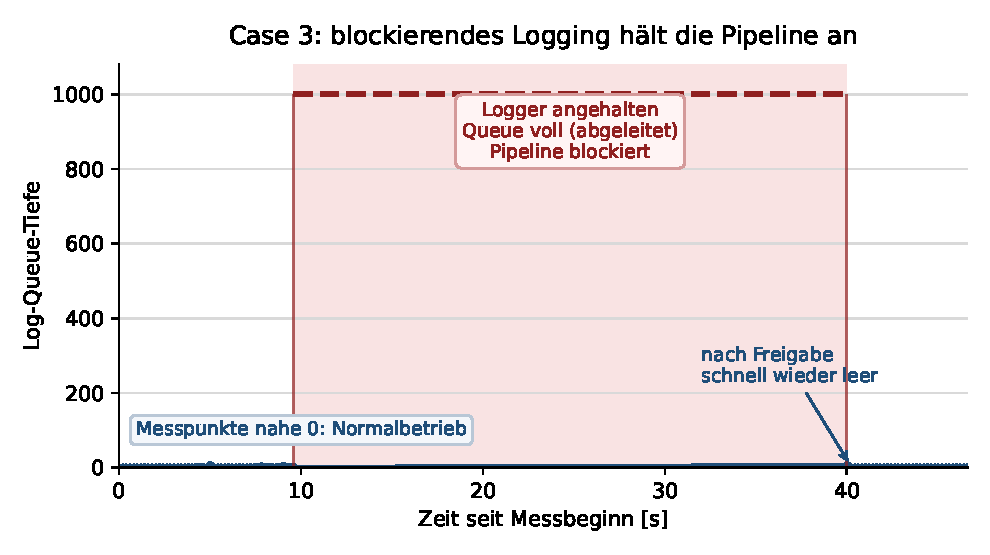
\includegraphics[width=0.85\textwidth]{assets/img/case3_queue_depth.pdf}
    \caption[Log-Queue bei angehaltenem Logger]{Log-Queue bei angehaltenem Logger. Die
        schattierte Phase enthält keine Messpunkte, weil der Logger-Prozess samt
        Mess-Thread pausiert. Aus dem anschließenden Rücksprung lässt sich ableiten, dass
        die Queue in dieser Phase vollgelaufen ist.}
    \source{Eigene Darstellung auf Basis eigener Messdaten}
    \label{fig:case3}
\end{figure}

Im Normalbetrieb bleibt die Queue nahezu leer. Wird der Logger angehalten, erreicht die
Queue ihre Kapazitätsgrenze; danach blockieren alle Prozesse, die beim nächsten Log-Aufruf
in diese Queue schreiben wollen. Der Stillstand entsteht also nicht in der Bildverarbeitung
selbst, sondern in einer gemeinsam genutzten Hilfskomponente. Nach Fortsetzung des Loggers
leert sich die Queue in unter 0,3~Sekunden. Der Engpass ist damit nicht die normale
Schreibgeschwindigkeit, sondern das blockierende Verhalten im Fehlerfall. Eine Umstellung
auf \texttt{put(timeout=0.1)} mit Drop-on-Full entkoppelt Logging und Pipeline: einzelne
Log-Einträge gehen verloren, die Verarbeitung bleibt jedoch lauffähig.

\subsection{Case 4 -- Veraltete Datenbankverbindung nach Produktionspause}
\label{sec:case4}

Die Persistierung der Inspektionsergebnisse erfolgt über das Django-ORM in der Funktion
\texttt{convert\_inspection\_to\_model}, die weder einen \texttt{OperationalError} abfängt
noch \texttt{close\_old\_connections()} aufruft. Entscheidend ist ein Konfigurationsgefälle
(Abschnitt~\ref{sec:grundlagen-parity}): Während die Entwicklung mit
\texttt{CONN\_\allowbreak{}MAX\_\allowbreak{}AGE = 0} pro Aufruf eine frische Verbindung
öffnet, hält die Produktion mit \texttt{CONN\_\allowbreak{}MAX\_\allowbreak{}AGE = 60} eine
persistente Verbindung. Zur Prüfung wurden in der Entwicklungsumgebung während des
Betriebs alle Datenbankverbindungen über \texttt{pg\_terminate\_backend} getrennt. Dieser
Versuch ist kein direkter Produktions-Crash-Test, sondern eine Negativkontrolle: Mit
\texttt{CONN\_\allowbreak{}MAX\_\allowbreak{}AGE = 0} öffnet Django pro Datenbankzugriff
eine neue Verbindung, sodass keine veraltete Verbindung entstehen kann. Vor dem Eingriff
waren rund 27 Inspektionen verarbeitet; 27 Datenbankverbindungen wurden terminiert. Das
System verarbeitete weiter, ein \texttt{OperationalError} trat nicht auf.

Das Risiko ergibt sich aus der Produktionskonfiguration. Nach einer Pause trennt
PostgreSQL oder eine vorgelagerte Firewall die inaktive Verbindung; der erste
Schreibzugriff danach trifft auf eine für gültig gehaltene, tatsächlich tote Verbindung
und löst einen \texttt{OperationalError} aus. Da dieser Fehler nicht behandelt wird, kann
der Worker abstürzen und über den bereits beschriebenen Mechanismus den PipelineManager
beenden. Der Fehler tritt damit beim ersten Materialdurchlauf nach einer Produktionspause
auf und wird durch die Entwicklungskonfiguration maskiert. Ein Aufruf von
\texttt{close\_old\_connections()} vor dem Schreibzugriff oder das Setzen von
\texttt{CONN\_\allowbreak{}MAX\_\allowbreak{}AGE = 0} auch in Produktion behebt das Problem;
die zusätzliche Latenz ist bei lokaler Datenbank vernachlässigbar
\cite{django_persistent_connections}.

\subsection{Case 5 -- Vermutete Race Condition im Speichermanagement}
\label{sec:case5}

Worker-Prozesse geben ihre Shared-Memory-Blöcke über eine Routine frei, die Blöcke nach
mehr als zehn Sekunden ohne Zugriff zerstört \cite{python_shm}. Die Ausgangshypothese
lautete, dass diese Freigabe unter Last Blöcke zerstören könnte, die der PipelineManager
noch benötigt, und so einen \texttt{FileNotFoundError} auslöst. Um den vermuteten Konflikt
zu provozieren, wurde die Freigabeschwelle von zehn auf zwei Sekunden gesenkt und ein
nachgelagerter Verarbeitungsschritt gezielt um vier Sekunden verzögert. Über 120~Sekunden
Laufzeit trat jedoch weder ein \texttt{FileNotFoundError} noch ein \texttt{BrokenPipeError}
oder ein Absturz auf.

Die Hypothese wird durch zwei Mechanismen widerlegt. Erstens greift der letzte lesende
Schritt typischerweise nach 45 bis 107~Millisekunden auf die Blöcke zu, während die
Freigabe frühestens nach zehn Sekunden erfolgt. Zweitens ist die Freigabeoperation
idempotent: Ein zweiter Aufruf liefert nur einen negativen Status zurück. Der vermutete
Pfad über einen langsamen Persistierungsschritt entfällt, weil dieser Schritt nicht auf
Shared-Memory-Blöcke zugreift. Für diesen Case besteht daher kein Sofortbedarf. Sinnvoll
bleiben ein Monitoring der Step-5-Laufzeit und langfristig ein Referenzzähler für
Speicherblöcke.
